\chapter{Umsetzung der interaktiven Benutzeroberfläche}
\label{chapter:umsetzung-der-interaktiven-benutzeroberfläche}

TODO:

\adjustbox{tabular=@{}l@{},width=\textwidth}{
\sffamily
Patchwork 1.0.0 (Debug Build) | Fabian Wolf \& Nico Zeitz                                                 \\
The board game Patchwork implemented in Rust with different AI players. Type "help" for more information. \\
> console                                                                                                  \\
Player 1: Human(name: Anonymer Modelleisenbahnliebhaber) \\
Player 2: Greedy \\
────────────────────────────────────────────────── TURN 1 ─────────────────────────────────────────────────── \\
Current player is 1                                                                                            \\
...                                                                                                            \\
\\
────────────────────────────────────────────────── TURN 13 ────────────────────────────────────────────────── \\
Current player is 1                                                                                           \\
\\
Player (button balance: 10): │ Player (button balance: 1):                                                    \\
░░░█████░                    │ ░░░░░░░░░                                                                      \\
███████░░                    │ ░░░░░░███                                                                      \\
█░░██░░░░                    │ ░░░░████░                                                                      \\
░░░░█░░░░                    │ ░░██████░                                                                      \\
░░░░░░░░░                    │ ░░███████                                                                      \\
░░░░░░░░░                    │ ░░██████░                                                                      \\
░░░░░░░░░                    │ ░░░█░░█░░                                                                      \\
░░░░░░░░░                    │ ░░░░░░░░░                                                                      \\
░░░░░░░░░                    │ ░░░░░░░░░                                                                      \\
Button income: 0             │ Button income: 3                                                               \\
\\
Time board:                                                                                                   \\
┌-┬-┬-┬-┬-┬-┬-┬-┬-┬-┬-┬-┬-┬-┬-┬-┬-┬-┬-┬-┬-┬-┬-┬-┬-┬-┬-┬-┬-┬-┬-┬-┬-┬-┬-┬-┬-┬-┬-┬-┬-┬-┬-┬-┬-┬-┬-┬-┬-┬-┬-┬-┬-┬-┐ \\
│ │ │ │ │ │B│ │ │ │ │ │B│ │ │ │1│2│B│ │ │ │ │ │B│ │ │P│ │ │B│ │ │P│ │ │B│ │ │P│ │ │B│ │ │P│ │ │B│ │ │P│ │ │B│ \\
└-┴-┴-┴-┴-┴-┴-┴-┴-┴-┴-┴-┴-┴-┴-┴-┴-┴-┴-┴-┴-┴-┴-┴-┴-┴-┴-┴-┴-┴-┴-┴-┴-┴-┴-┴-┴-┴-┴-┴-┴-┴-┴-┴-┴-┴-┴-┴-┴-┴-┴-┴-┴-┴-┘ \\
Next 6 patches (can only take first 3): \\
█                                                     █                ██  \\
█                                                     █                ██  \\
█                  █               ██                ██                 █                  █  \\
███               ███               ██                █                  █                 ██  \\
Id: 12            Id: 19            Id: 9             Id: 10            Id: 13             Id: 21  \\
Income: 2         Income: 1         Income: 2         Income: 1         Income: 3          Income: 0  \\
Button cost: 7    Button cost: 4    Button cost: 6    Button cost: 2    Button cost: 10    Button cost: 1  \\
Time cost: 2      Time cost: 2      Time cost: 5      Time cost: 3      Time cost: 5       Time cost: 3  \\
\\
Player 'HumanPlayer(name: Anonymer Modelleisenbahnliebhaber)' can choose one of the following actions: 'take 1', 'take 2', 'take 3', 'walk'. Please enter the action: take 2 \\
You chose to place the following patch: \\
█   Id: 19 \\
███ Income: 1 \\
Button cost: 4 \\
Time cost: 2          \\
Please enter the  rotation (0, 90, 180, 270) and orientation (if flipped: y/n) of the patch: 0,n \\
Please enter the row and column of the patch (row, column): 5,5 \\
Player 'HumanPlayer(name: Anonymer Modelleisenbahnliebhaber)' chose action: Action 402 - Patch(12) placement (index 0) at (4, 4) with (R 0°, O normal) (P12I0═4‖4↻0↔0P1) after 15.95s \\
}

TODO:

\begin{figure}[!ht]
    \centering
    \begin{tikzpicture}
        \node [inner sep=0pt,,outer sep=0pt,clip,rounded corners=0.15cm] (image) at (0,0) {
            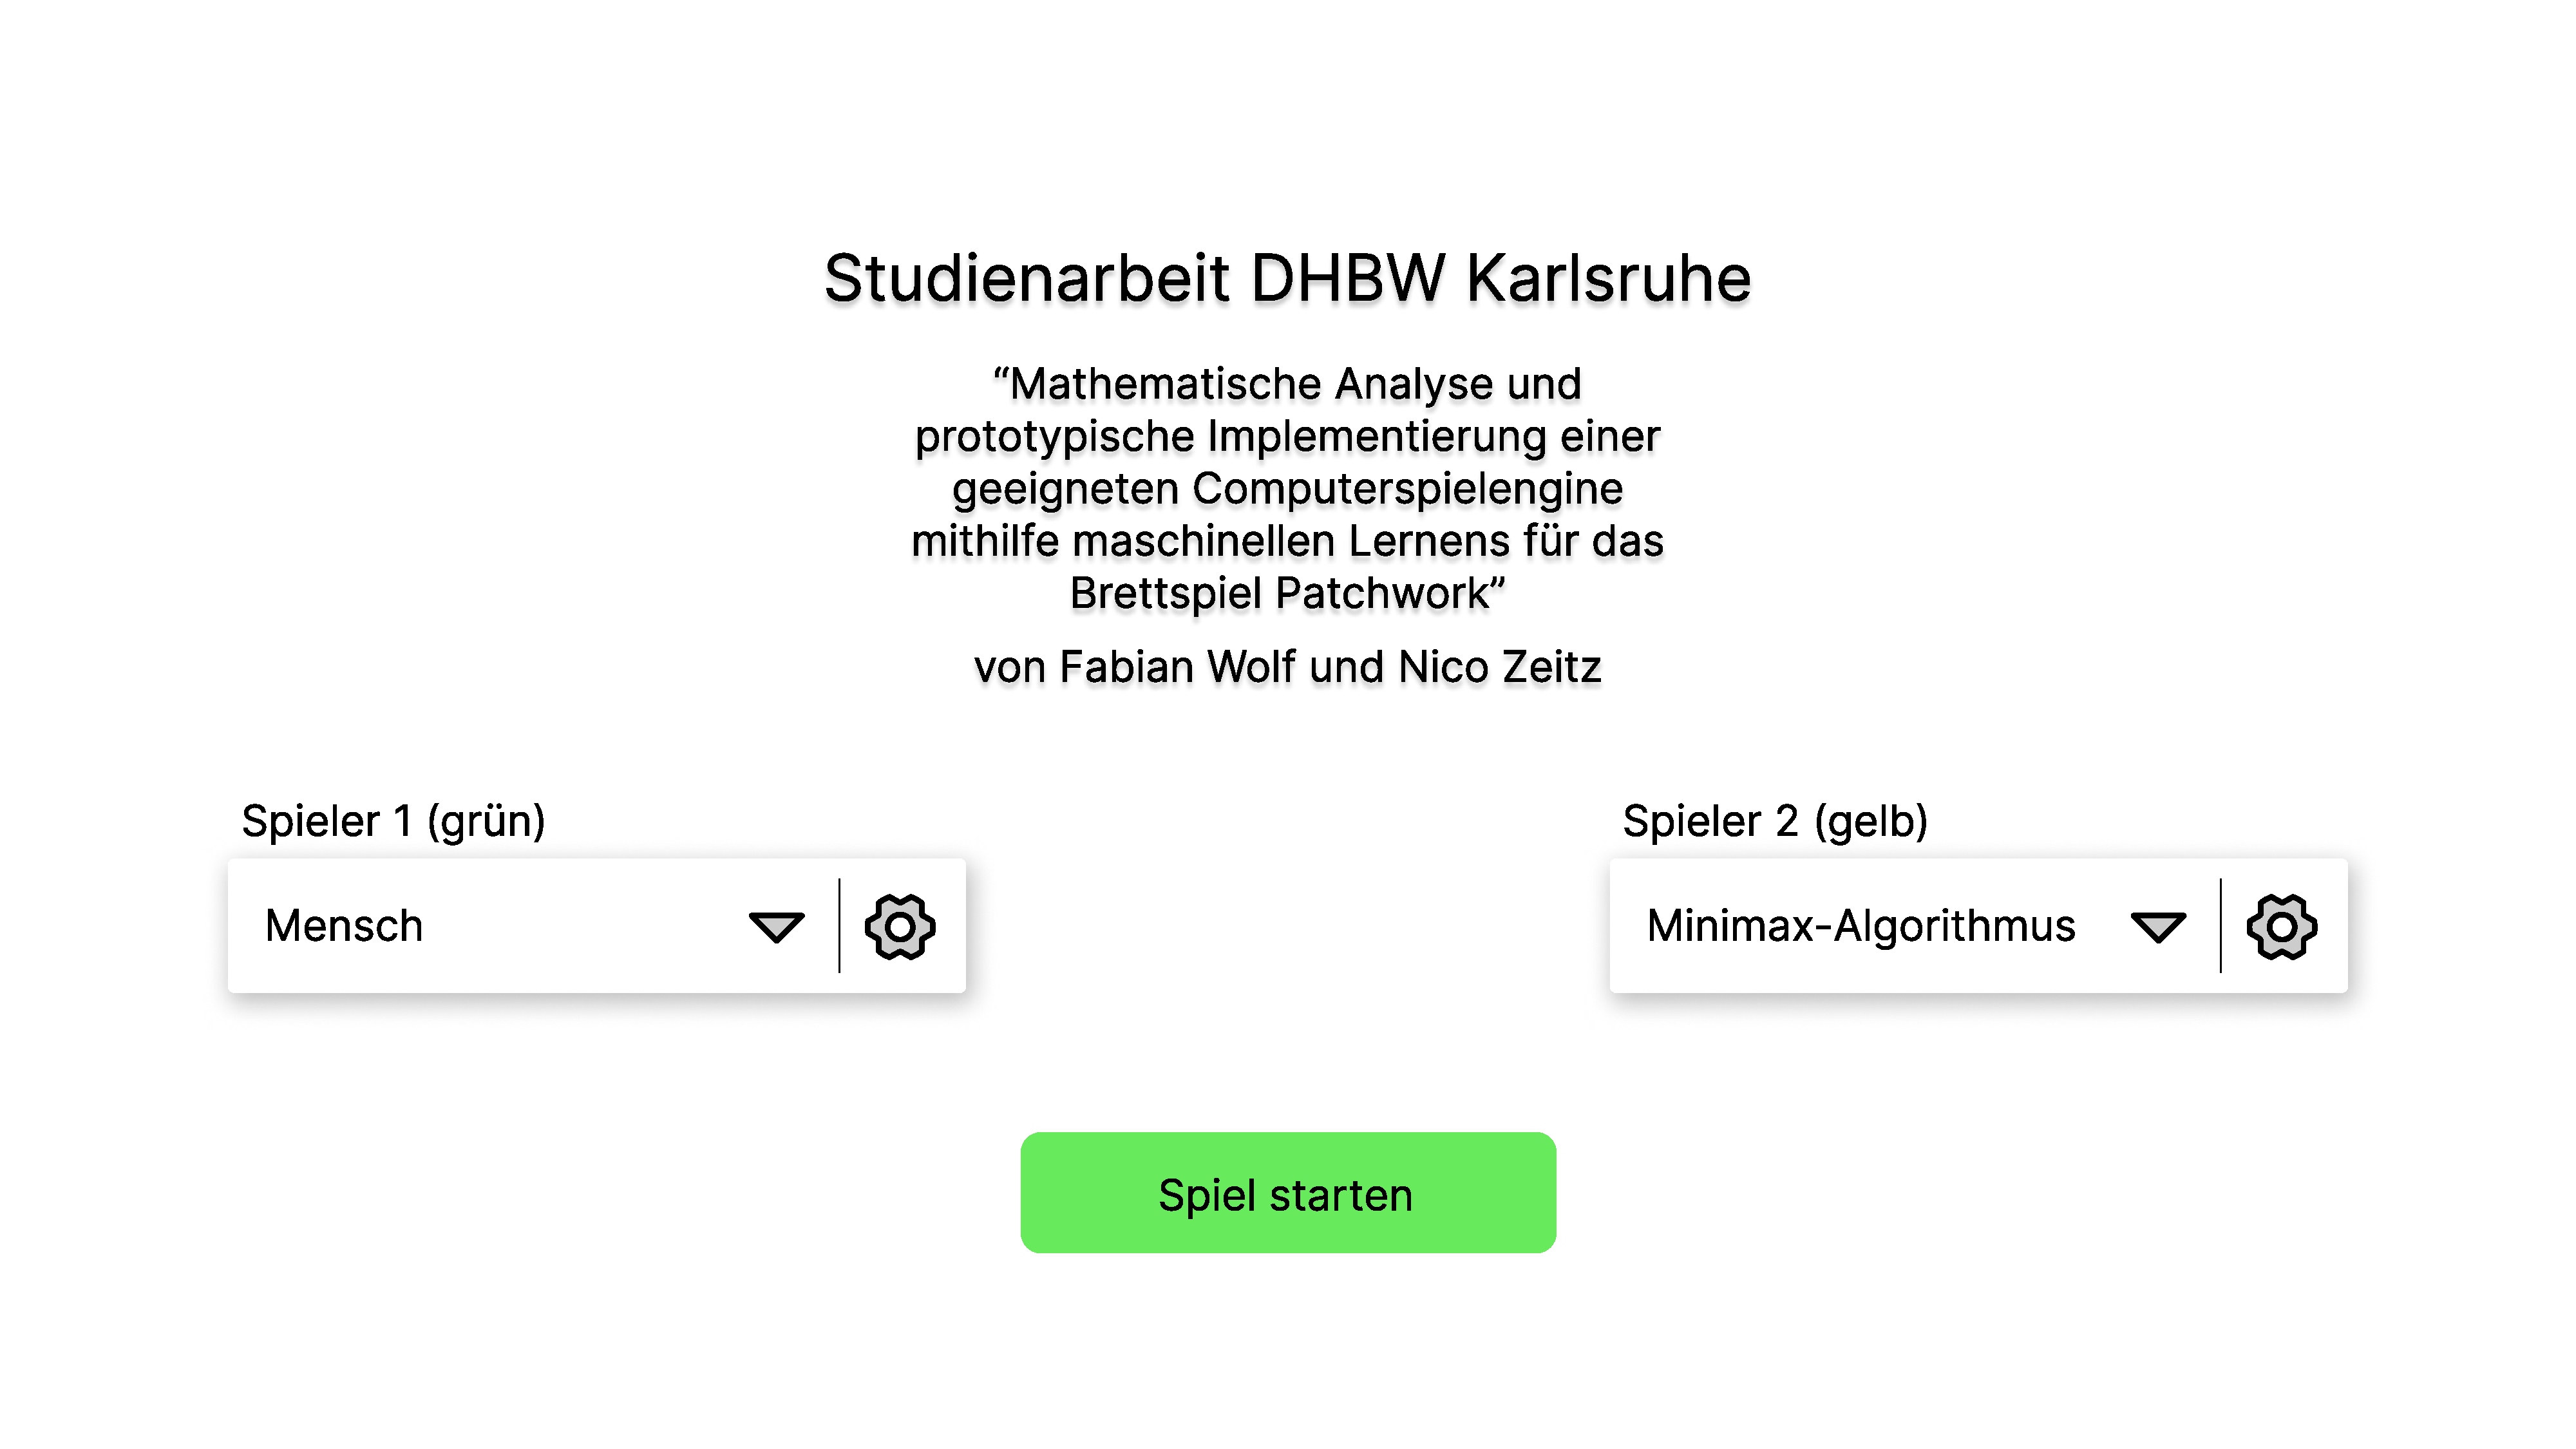
\includegraphics[width=\textwidth]{res/pictures/desig_main_ui.pdf}};
        \drawshadow{image}
    \end{tikzpicture}
    \caption{Designentwurf vom Hauptmenü des Computerspiel}
    \label{fig:design-main-ui}
\end{figure}

\begin{figure}[!ht]
    \centering
    \begin{tikzpicture}
        \node [inner sep=0pt,,outer sep=0pt,clip,rounded corners=0.15cm] (image) at (0,0) {
            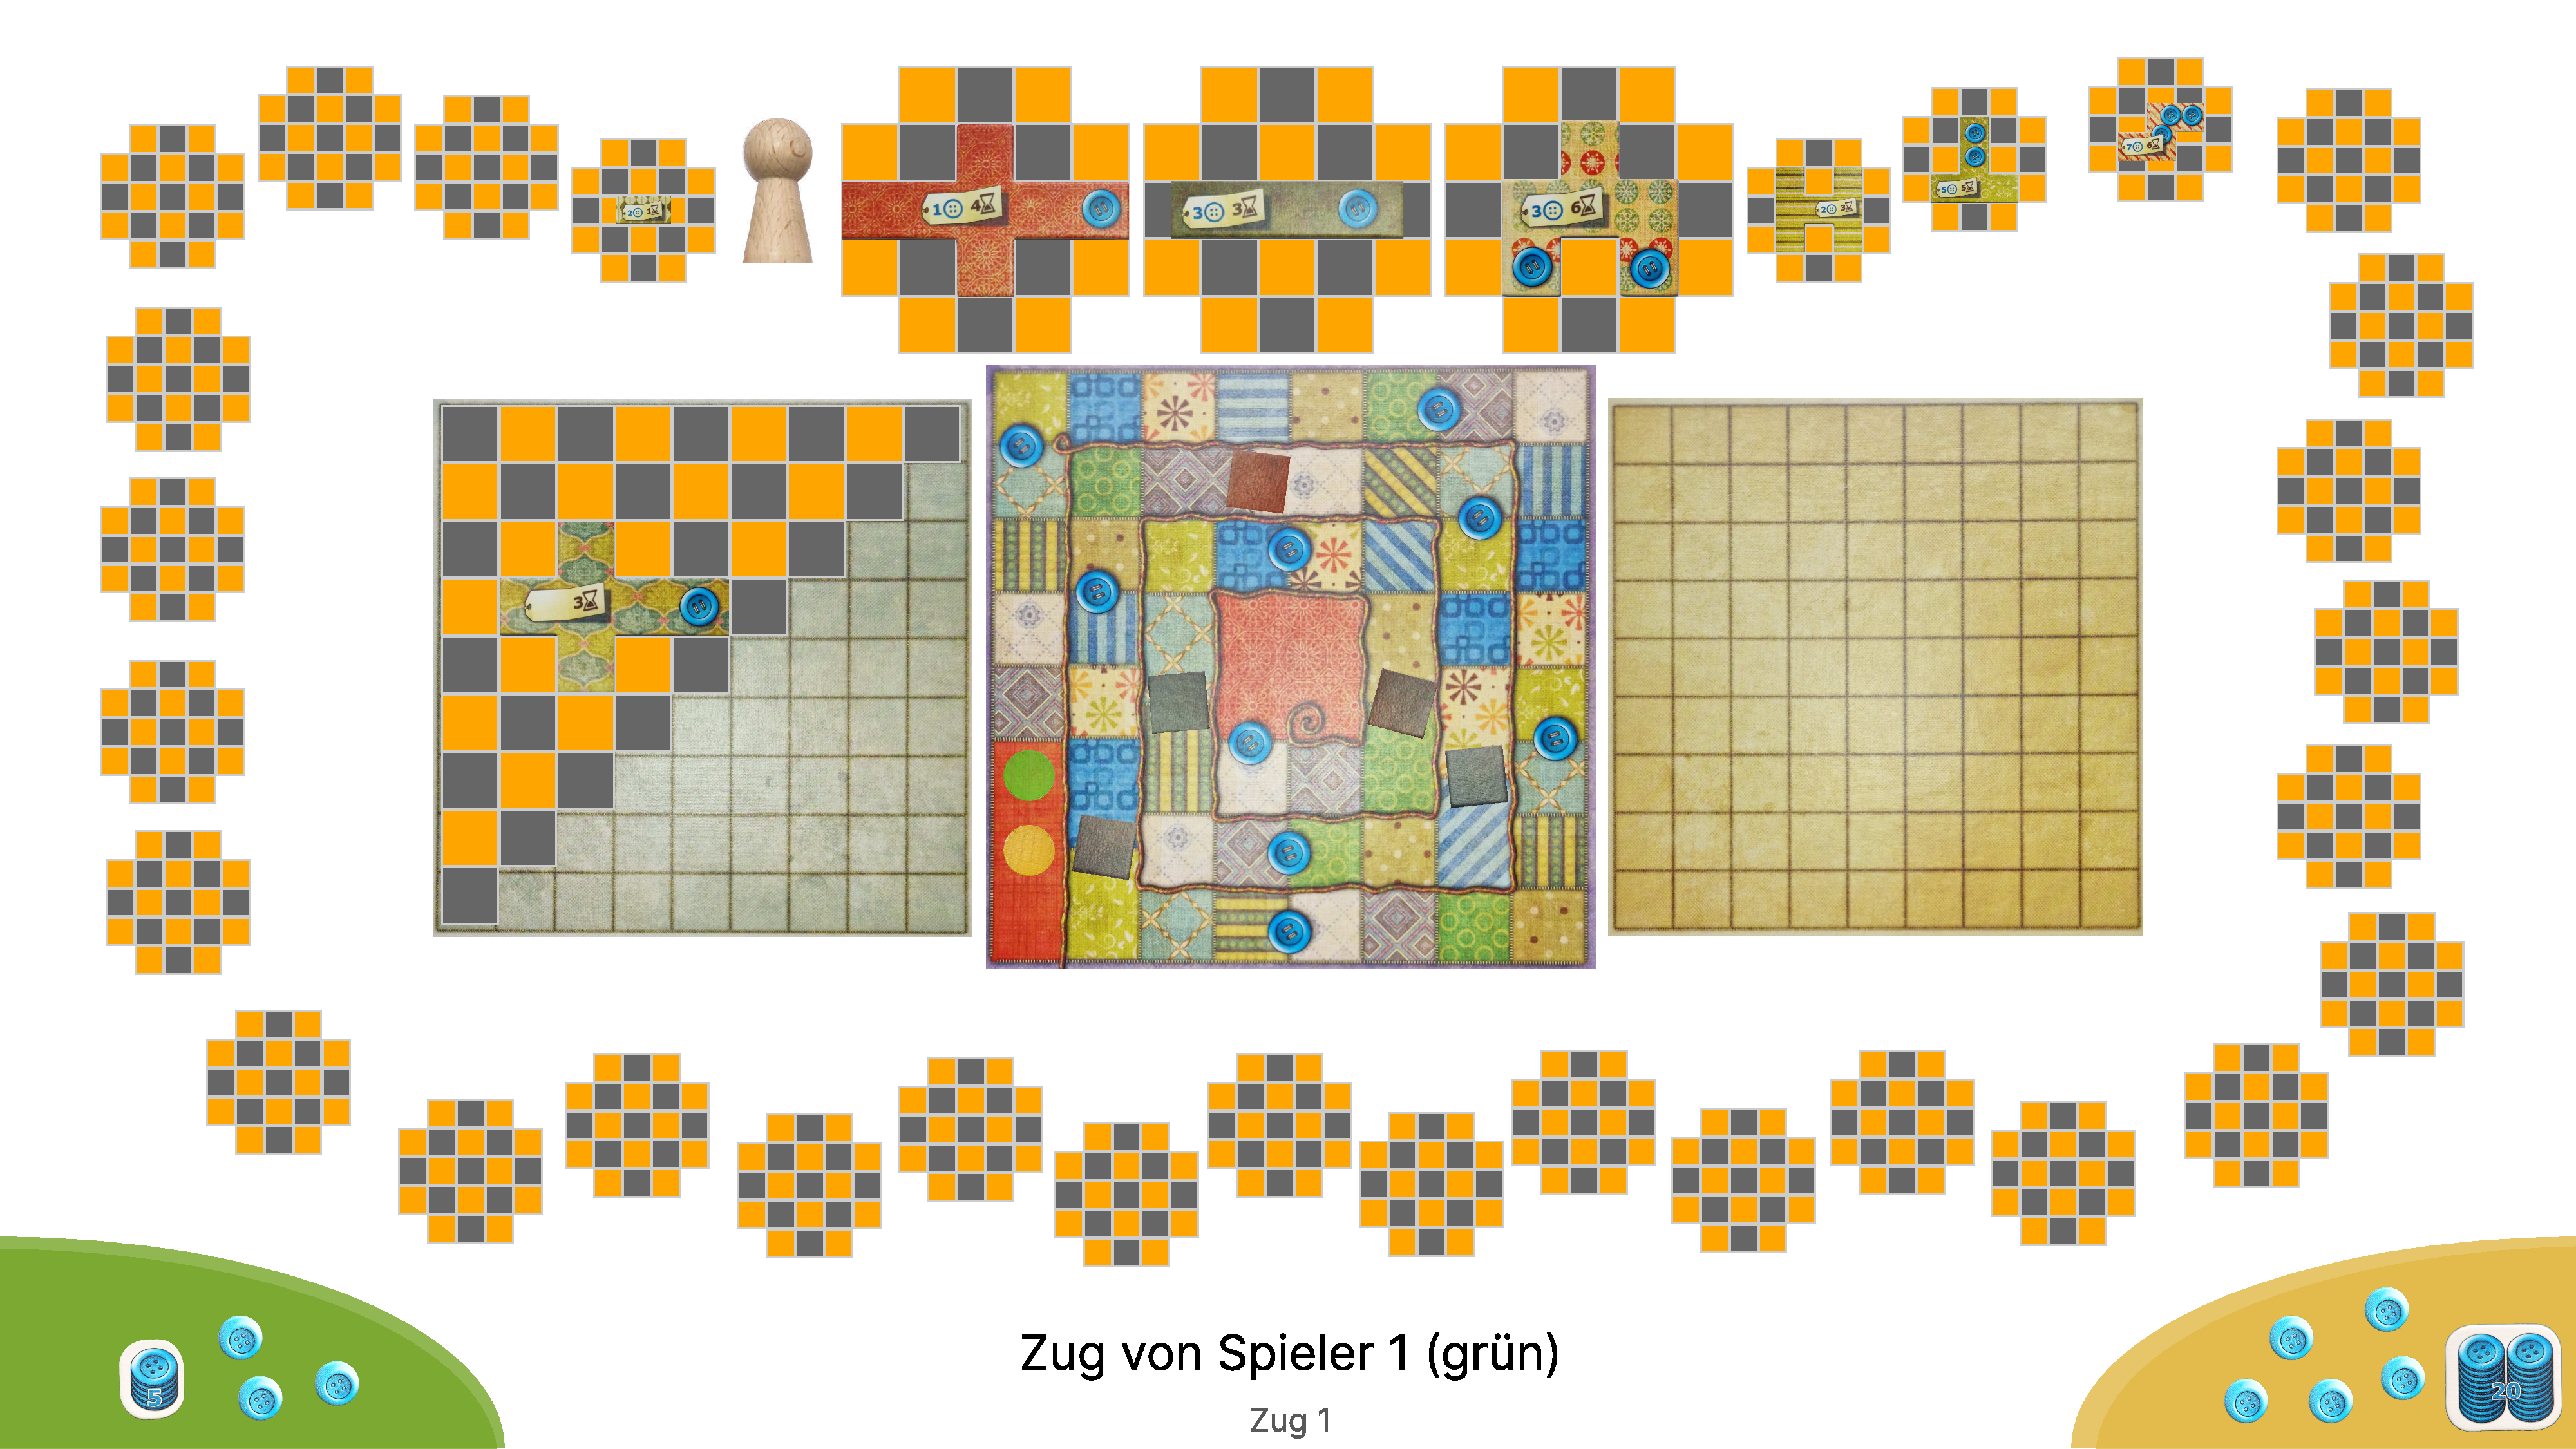
\includegraphics[width=\textwidth]{res/pictures/design_game_ui.pdf}};
        \drawshadow{image}
    \end{tikzpicture}
    \caption{Designentwurf der grafische Benutzeroberfläche des Computerspiel}
    \label{fig:design-game-ui}
\end{figure}



\begin{figure}[!ht]
    \centering
    \begin{tikzpicture}
        \node [inner sep=0pt,,outer sep=0pt,clip,rounded corners=0.15cm] (image) at (0,0) {
            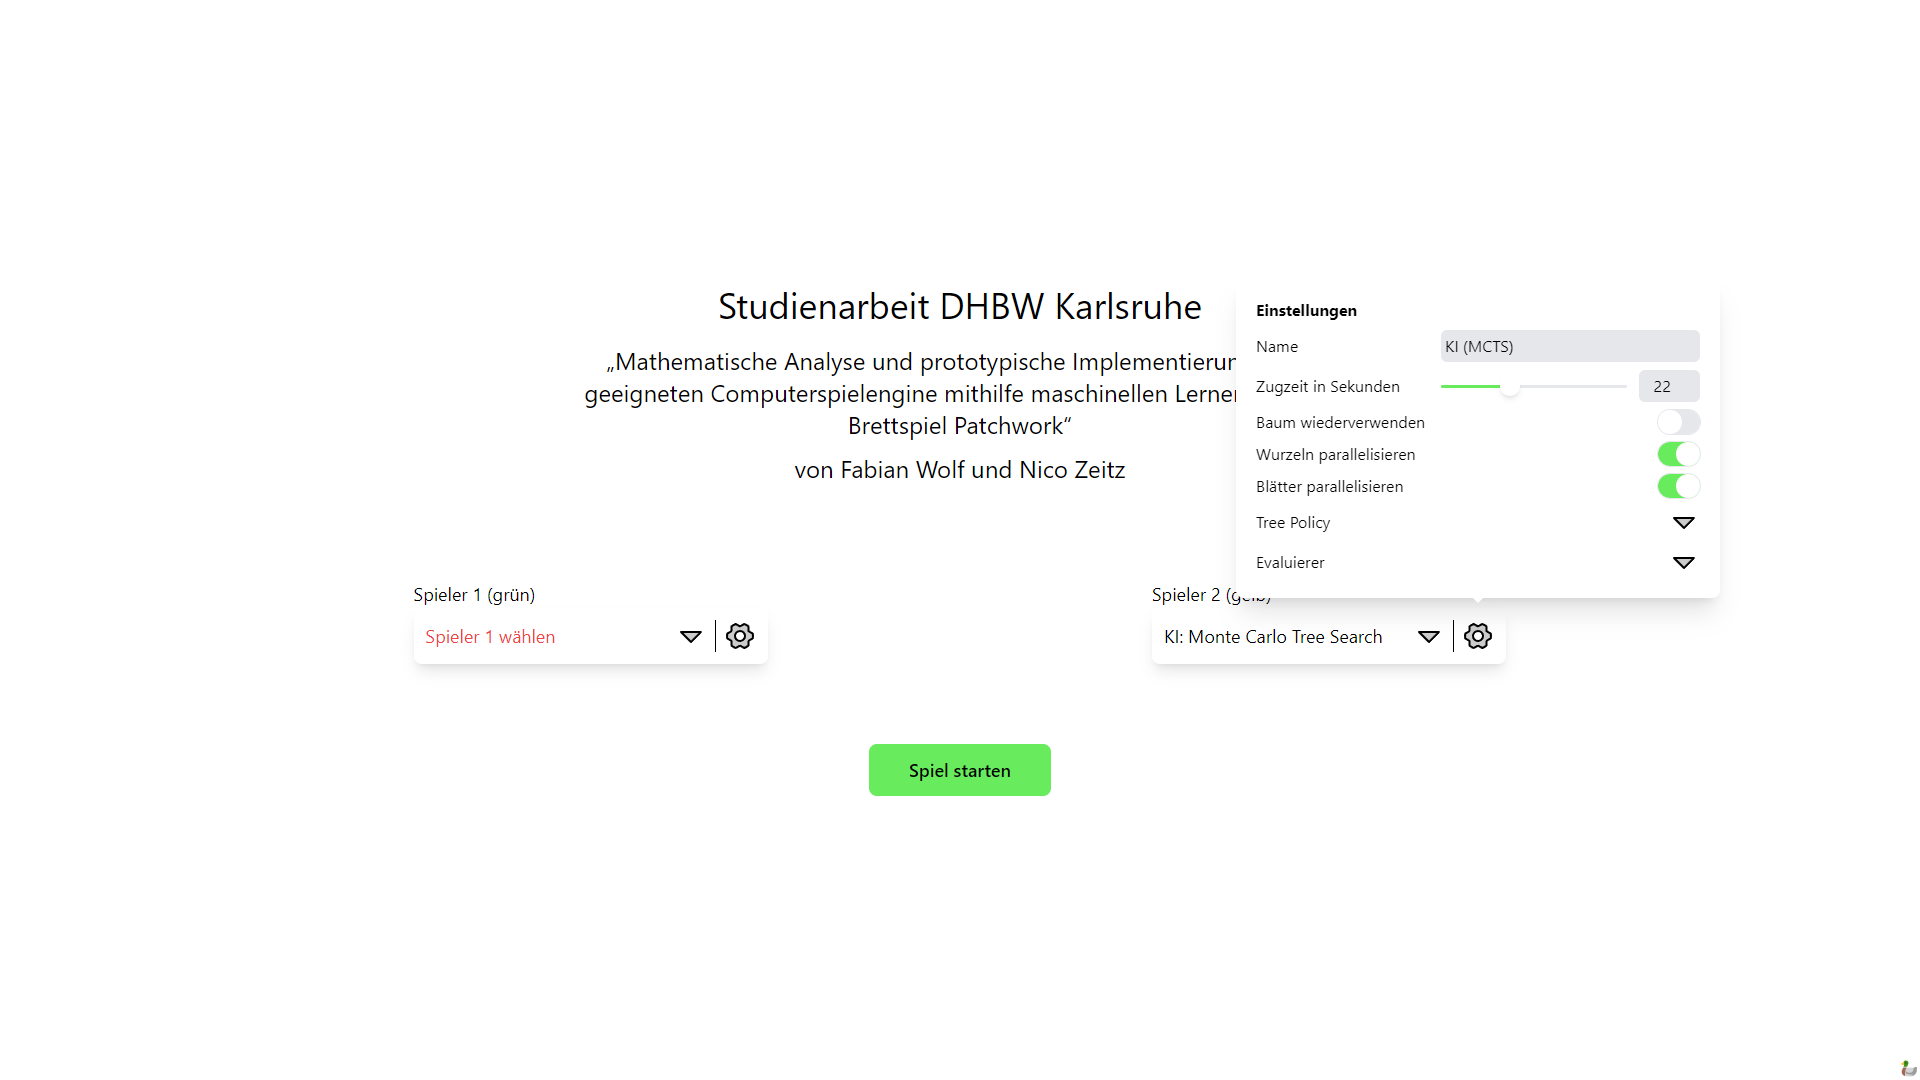
\includegraphics[width=\textwidth]{res/pictures/final_main_ui.png}};
        \drawshadow{image}
    \end{tikzpicture}
    \caption{Umsetzung des Hauptmenü des Computerspiel}
    \label{fig:final-main-ui}
\end{figure}



\begin{figure}[!ht]
    \centering
    \begin{tikzpicture}
        \node [inner sep=0pt,,outer sep=0pt,clip,rounded corners=0.15cm] (image) at (0,0) {
            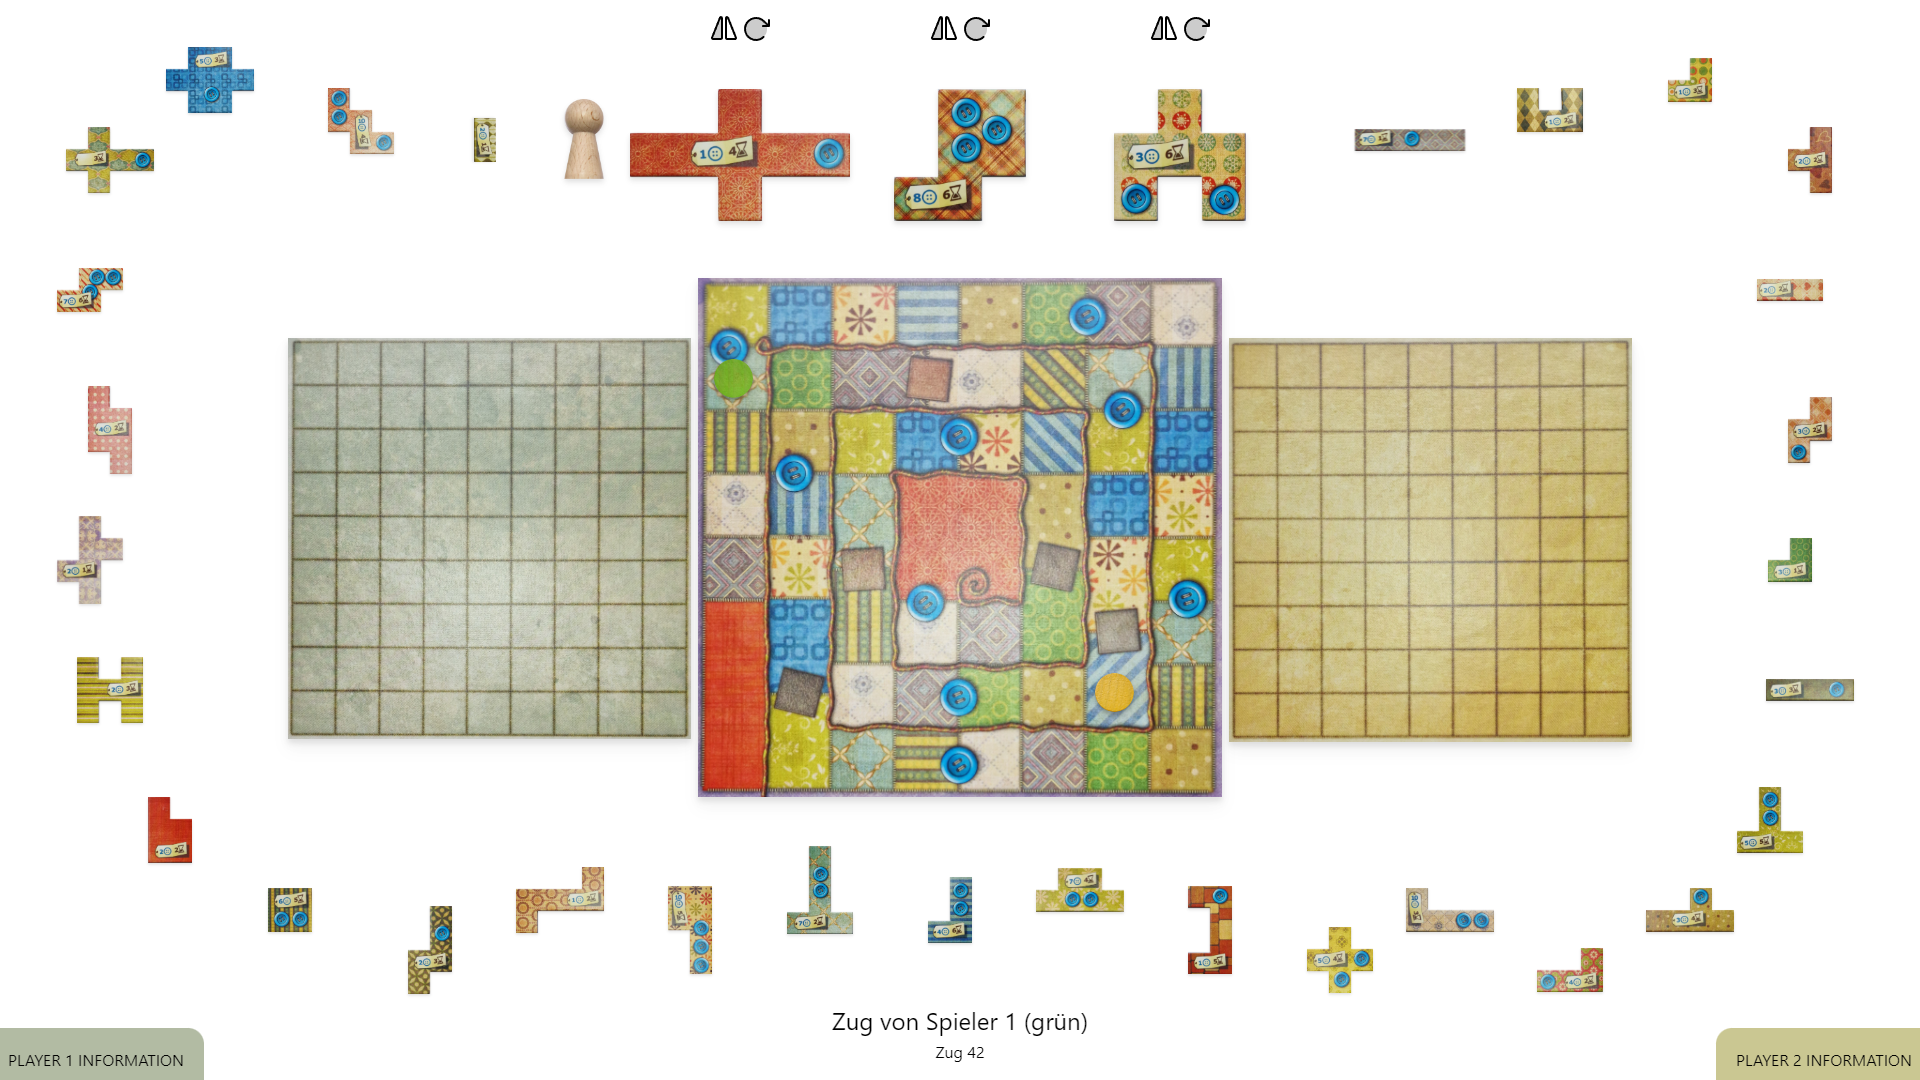
\includegraphics[width=\textwidth]{res/pictures/final_game_ui.png}};
        \drawshadow{image}
    \end{tikzpicture}
    \caption{Umsetzung der grafische Benutzeroberfläche des Computerspiel}
    \label{fig:final-game-ui}
\end{figure}